\section{Diskussion}
\label{sec:Diskussion}
\begin{figure}
    \centering
    \begin{minipage}{.5\textwidth}
        \centering
        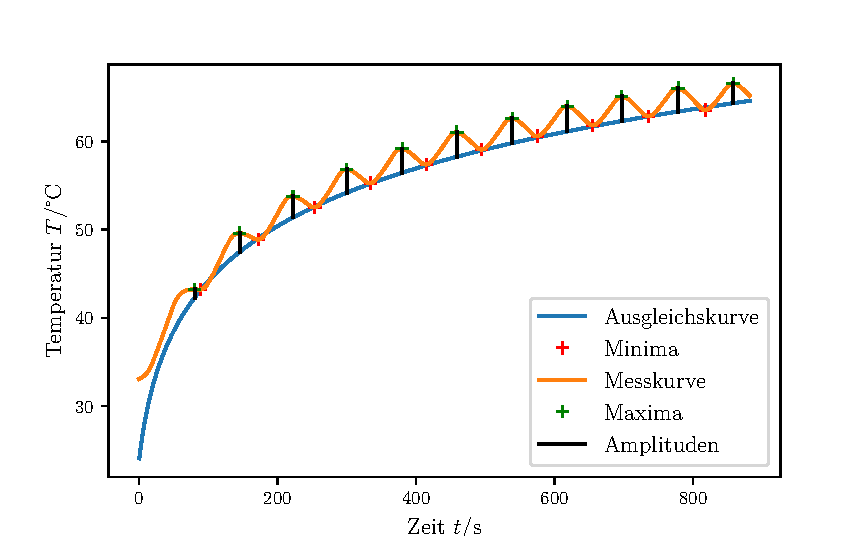
\includegraphics[max width=1.1\linewidth]{plots/amplitudes_brass_wide_far(t1).pdf}
        \caption{}
        \label{fig:plot_amps_t1}
    \end{minipage}%
    \begin{minipage}{.5\textwidth}
        \centering
        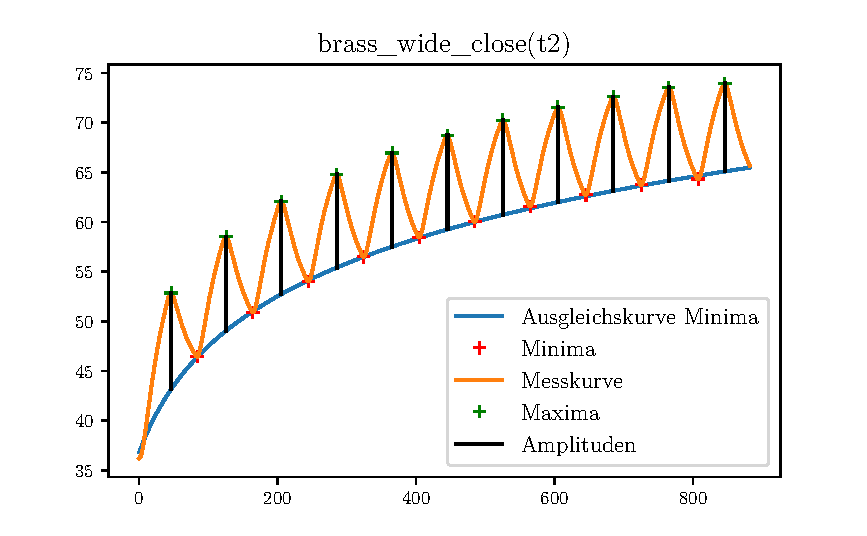
\includegraphics[max width=1.1\linewidth]{plots/amplitudes_brass_wide_close(t2).pdf}
        \caption{}
        \label{fig:plot_amps_t2}
    \end{minipage}
    \caption{Messwertanalyse zu T1 und T2, Messing(breit), fern und nah.}
    \label{fig:plots_amps_t1_t2}
\end{figure}

\begin{table}
    \centering
    \caption{Amplituden von Messing, nah und fern, in $\si{\kelvin}$.}
    \label{tab:amps_brass}
    \begin{tabular}{S[table-format=3.1] S[table-format=1.2] | S[table-format=3.1] S[table-format=1.2]}
        \toprule
        \multicolumn{2}{c}{$\symup{Messing}_\text{nah}$} & \multicolumn{2}{c}{$\symup{Messing}_\text{fern}$} \\
        \cmidrule(lr){1-2}\cmidrule(lr){3-4}
        {$t[\si{\s}]$} & {$\increment T[{\si{\kelvin}]}$} & {$t[\si{\s}]$} & {$\increment T[{\si{\kelvin}]}$} \\
        \midrule
         46.5 &	9.70 &    80.5 & 0.91 \\	
        126.0 &	9.47 &   145.5 & 2.11 \\		
        205.5 &	9.36 &   222.5 & 2.39 \\		
        285.5 &	9.38 &   300.0 & 2.63 \\		
        365.5 &	9.43 &   380.0 & 2.72 \\		
        445.5 &	9.46 &   459.0 & 2.78 \\		
        525.5 &	9.53 &   539.0 & 2.81 \\		
        605.0 &	9.57 &   618.5 & 2.84 \\		
        685.0 &	9.47 &   697.0 & 2.78 \\		
        765.0 &	9.40 &   778.5 & 2.65 \\
        \bottomrule
    \end{tabular}
\end{table}